\newcommand{\NUMBER}{8}
\newcommand{\EXERCISES}{2}
\newcommand{\DEADLINE}{6.22.21}
\newcommand{\COURSE}{Data Compression}
\newcommand{\STUDENTA}{Philipp von Bachmann, 4116220}
\newcommand{\STUDENTB}{Jessica Bader, 5624582}
\documentclass[a4paper]{scrartcl}
\usepackage[utf8]{inputenc}
\usepackage[english]{babel}
\usepackage{amsmath, enumerate, amssymb, multirow, fancyhdr, color, graphicx, lastpage, listings, tikz, pdflscape, subfigure, float, polynom, hyperref, tabularx, forloop, geometry, listings, fancybox, tikz, forest, tabstackengine, cancel}
\input kvmacros
\geometry{a4paper,left=3cm, right=3cm, top=3cm, bottom=3cm}
\pagestyle {fancy}
\fancyhead[C]{\COURSE}
\fancyhead[R]{\today}
\fancyfoot[L]{}
\fancyfoot[C]{}
\fancyfoot[R]{Page \thepage /\pageref*{LastPage}}
\def\header#1#2{
  \begin{center}
    {\Large Progress Update: Jun. 22}\\
    %{(Due by: #2)}
  \end{center}
}

\begin{document}

\begin{tabularx}{\linewidth}{m{0.3 \linewidth}X}
  \begin{minipage}{\linewidth}
    \STUDENTA\\
    \STUDENTB
  \end{minipage}
\end{tabularx}
\header{Progress Update}{\DEADLINE}
\section{Planning}
We have designed three possible architectures for our project (see figures 1-3). We plan to start working with the first two simultaneously. These architectures assume that state space of the RL agent is helpful as a latent space; if this proves to be incorrect, we will change to architecture 3.\\
We have identified the Multi-scale Structural Similarity metric as our ideal metric, as it is commonly used in literature and preferred over MSE as a 'human centered' metric.\\
We have decided to first compare our method with standard compression algorithms (BPG, WebP, JPEG) as found in several published pieces of literature, in terms of bits per dimension of similarly accurate evaluation on the reconstructed image of an RL agent trained on the original images. We have also identified several SOTA compression techniques ($\delta$-VAE, NVAE, etc.) to compare with if time and algorithm success allow.\\
We chose the Atari game suite as our data set, starting with Breakout.
\section{Implementation}
We implemented the most basic version of Architecture 1 for Breakout from gym, which uses states/images of size $3\cdot210\cdot160$. We converted them to greyscale, resulting in a flattened size of 33,600. We then trained a standard RL agent (PPO) to play the game for 10,000 environment steps. As it trained, we saved 1,000 random states as the original image with its corresponding state value function, having a latent space of 128 dimensions. After training, these were passed to a single layer, fully connected NN decoder which used MSE between the original image and latent space as a loss function for 1,000 epochs. To compare, we used the same training for the decoder, but with an untrained RL agent. The results in Figure \ref{fig:train_results} show that not only is the decoder able to learn, but it also performs better if a pre-trained agent is used. This shows that in a very simple model, the RL agent provides at least some valuable information to the decoder.

\begin{figure}[H]
    \centering
    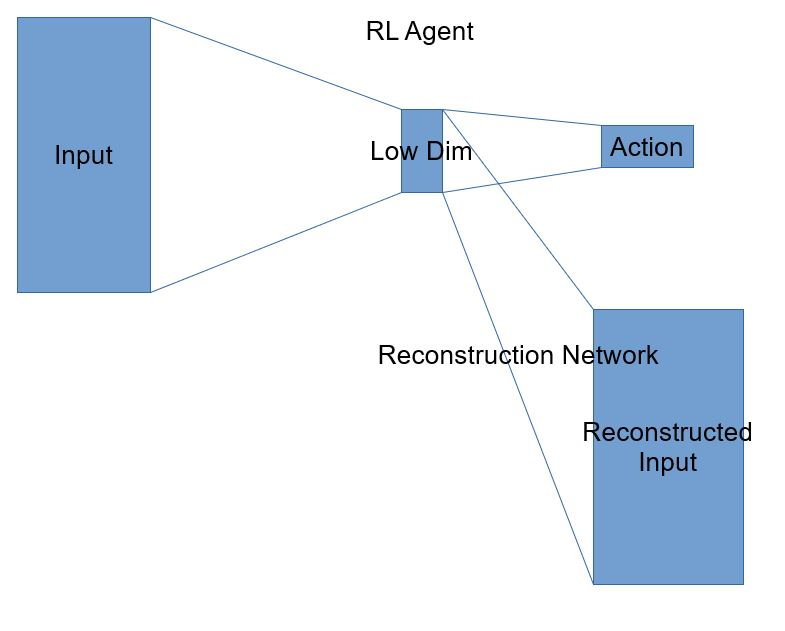
\includegraphics[width=0.6\textwidth]{Arch1.JPG}
    \caption{First architecture (simplest)}
    \label{fig:arch1}
\end{figure}
\begin{figure}[H]
    \centering
    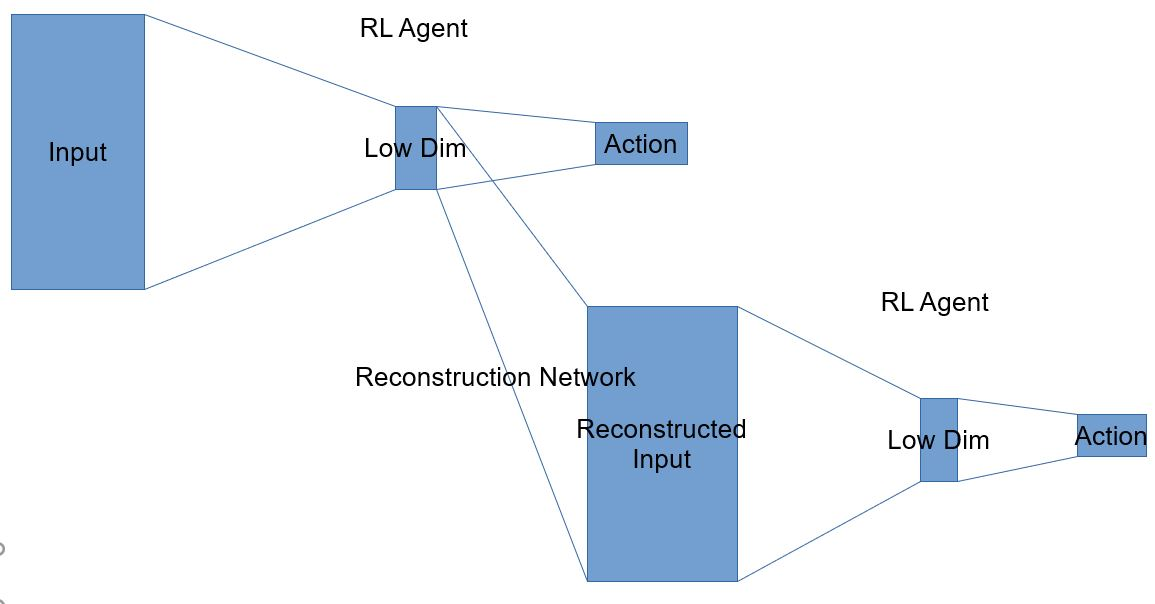
\includegraphics[width=0.6\textwidth]{Arch2.JPG}
    \caption{Second architecture}
    \label{fig:arch2}
\end{figure}
\begin{figure}[H]
    \centering
    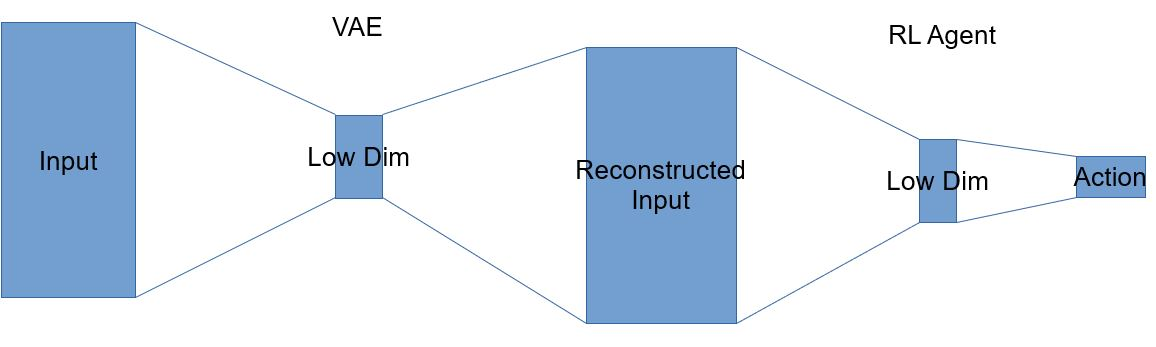
\includegraphics[width=0.6\textwidth]{Arch3.JPG}
    \caption{Third architecture (avoids state space assumption)}
    \label{fig:arch3}
\end{figure}


  \begin{figure}[H]
    \centering
    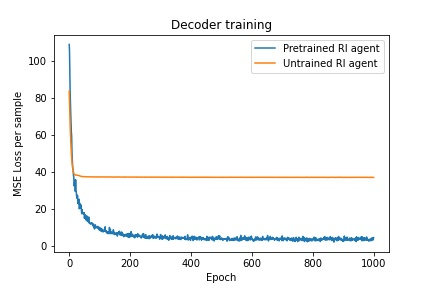
\includegraphics[width=0.5\textwidth]{training_results.jpg}
    \caption{Training results}
    \label{fig:train_results}
\end{figure}
\end{document}